%!TEX program =pdflatex
\documentclass{beamer}
\usetheme{CambridgeUS}
%%define new comand
\def\argmin{\mathop{\rm arg~min}\limits}
\def\argmin{\mathop{\rm arg~min}\limits}
\newcommand{\bdelta}{\boldsymbol{\delta}}
\newcommand{\bbeta}{\boldsymbol{\beta}}
\newcommand{\bSigma}{\boldsymbol{\Sigma}}
\newcommand{\brho}{\displaystyle{\large{\boldsymbol{\rho}}}}
\newcommand{\bgamma}{\boldsymbol{\gamma}}
\newcommand{\bfeta}{\boldsymbol{\eta}}
\newcommand{\bPsi}{\boldsymbol{\Psi}}
\newcommand{\bmu}{\boldsymbol{\mu}}
\newcommand{\bvartheta}{\boldsymbol{\vartheta}}
\newcommand{\bzero}{\mathbf{0}}
\newcommand{\bone}{\mathbf{1}}
\newcommand{\bA}{\mathbf{A}}
\newcommand{\ba}{\mathbf{a}}
\newcommand{\bB}{\mathbf{B}}
\newcommand{\bb}{\mathbf{b}}
\newcommand{\bD}{\mathbf{D}}
\newcommand{\bU}{\mathbf{U}}
\newcommand{\bu}{\mathbf{u}}
\newcommand{\bV}{\mathbf{V}}
\newcommand{\bW}{\mathbf{W}}
\newcommand{\bw}{\mathbf{w}}
\newcommand{\bX}{\mathbf{X}}
\newcommand{\bx}{\mathbf{x}}
\newcommand{\bY}{\mathbf{Y}}
\newcommand{\by}{\mathbf{y}}
\newcommand{\bZ}{\mathbf{Z}}
\newcommand{\bz}{\mathbf{z}}
\newcommand{\suit}[1]{\left(#1\right)}
\newcommand{\abs}[1]{\left\vert#1\right\vert}
\newcommand{\set}[1]{\left\{#1\right\}}
\newcommand{\msuit}[1]{\left[ #1 \right]}
\author{Y. He, Y. Hou, L. Peng and J. Sheng}
\title{Statistical Inference for a Relative Risk Measure}
\begin{document}
\begin{frame}
\titlepage
\vspace{-3ex}
\begin{center}
    Published by Journal of Business and Economics Statistics (2009).

    \bigskip

    Presented by Liujun Chen.
\end{center}
\end{frame}
\AtBeginSection[]
{
\begin{frame}
\frametitle{Table of Contents}
\tableofcontents[currentsection]
\end{frame}
}


\section{Introduction}
\begin{frame}
    \frametitle{Systemic Risk}
\begin{itemize}
    \item A formal definition of systemic risk does not exist arguably.
    \bigskip
    \item It is
    commonly agreed that systemic risk involves the co-movement
    of several key financial variables. 
    \bigskip
    \item Many measures have been
    proposed in the literature.
\end{itemize}    

\end{frame}



\begin{frame}
    \frametitle{Relative Risk Measure}
\begin{itemize}
    \item From regulators’ point of view, having risk measures from     each agency does not help understand/measure systemic risk     at all.
  \medskip
    \item It would be more meaningful to have some
    relative risk measures reported by each agency with respect to 
    a common benchmark.
\end{itemize}
    
\bigskip
Therefore, an interesting question becomes:
\medskip
\begin{itemize}
    \item[(a)] how to define a relative risk measure, which should be quite    sensitive to the market co-movement for the purpose of studying    systemic risk
    \medskip
    \item[(b)] how to infer such a relative risk measure. 
\end{itemize}
\end{frame}

\begin{frame}
    \frametitle{Mathematical Definition}
\begin{itemize}
    \item Let $X$ denote the loss of an individual portfolio; $Y$ denote the loss of some benchmark (a financial market index). 
    \item Consider the commonly employed expected shortfall
    risk measure at level $\alpha \in (0,1)$, defined as
    $$
    \begin{aligned}
        \text{ES}_{\alpha}(X)&=E[X|F_1(X)>1-\alpha] \\
        \text{ES}_{\alpha}(Y)&=E[Y|F_2(X)>1-\alpha]
    \end{aligned}
    $$
    \item A quick
    way to compare these two risk measures is to look at their ratio
    $$
            \frac{\text{ES}_{\alpha}(X)}{\text{ES}_{\alpha}(Y)}
    $$
\end{itemize}

\end{frame}

\begin{frame}
    \frametitle{Relative Risk}
\begin{itemize}
    \item this ratio  is invariant to the copula of X and Y , that is, it is irrelevant to the market comovement.
    \item To capture the extreme
    dependence between $X$ and $Y$, Agarwal et al.(2017) proposed to multiply the above ratio by the
    coefficient of (upper) tail dependence 
    $$
        \lambda = \lim_{t \downarrow 0} P\suit{F_1(x)>1-t|F_2(Y)>1-t}.
    $$
    \item Since the coefficient of tail dependence
    is defined in a limiting way, nonparametric estimator for it has
    a slower rate of convergence than that for the ratio of expected
    shortfalls.
\end{itemize}
    

\end{frame}

\begin{frame}
    \frametitle{Relative Risk}
    \begin{itemize}
        \item Agarwal et al.(2017)  proposes to define the relative risk as
        $$
\rho_{\alpha}=\rho_{\alpha}(X,Y)=P\suit{F_1(x)>1-\alpha|F_2(Y)>1-\alpha} \frac{\text{ES}_{\alpha}(X)}{\text{ES}_{\alpha}(Y)}
        $$
        \item This article aims to derive asymptotic
        limit for a nonparametric estimator and its smoothed version of
        the above relative risk measure and to provide an effective way
        to construct an interval by considering either a fixed level or an
        intermediate level.
    \end{itemize}
    
\end{frame}


\section{Main Results For Independent Data}

\begin{frame}
    \frametitle{Notations}
\begin{itemize}
    \item Let $(X_1,Y_1), \dots, (X_n,Y_n)$ be i.i.d. random vectors with joint d.f. $F(x,y)$ and marginals $F_1,F_2$. 
    \item Order the $X_i$'s as $X_{1,n}\le X_{2,n}\le \cdots\le X_{n,n}$ and $Y_i$'s as $Y_{1,n}\le Y_{2,n}\le \cdots\le Y_{n,n}$.
    \item $\bar{F}_i=1-F_i$ and $Q_i=F_i^{\leftarrow}$.
    \item Use $\bar{F}_{n1}(x)$ and $\bar{F}_{n2}(y)$ denote the empirical survival function of $X$ and $Y$ respectively.
    \item Define survival copula function
        $$
            C(u,v)=P\suit{\bar{F}_1(X)<u, \bar{F}_2(Y)<v}.
        $$
\end{itemize}
\end{frame}


\begin{frame}
    \frametitle{Non-parametric Estimation}
We can rewrite 
$$
\rho_{\alpha}=\frac{1}{\alpha}C(\alpha,\alpha)\frac{\text{ES}_{\alpha}(X)}{\text{ES}_{\alpha}(Y)}.
$$
Substituting the right-hand-side components by their empirical
counterparts yields our nonparametric estimator
$$
\rho_{\alpha}=\frac{1}{\alpha}\widetilde{C}(\alpha,\alpha)\frac{\widetilde{\text{ES}}_{\alpha}(X)}{\widetilde{\text{ES}}_{\alpha}(Y)}.
$$

\end{frame}

\begin{frame}
    \frametitle{Smoothed Estimator}
  With some density function $k$, its distribution function $K$ and the bandwidth $h=h(n)>0$, a smoothed estimator of $\rho_{\alpha}$ is given by
    $$
    \rho_{\alpha}=\frac{1}{\alpha}\widehat{C}(\alpha,\alpha)\frac{\widehat{\text{ES}}_{\alpha}(X)}{\widehat{\text{ES}}_{\alpha}(Y)},
    $$
    where
    $$
        \begin{aligned}
        \widehat{C}(\alpha,\alpha)&= \frac{1}{n}\sum_{j=1}^n K\suit{\frac{1-\bar{F}_{n1}(X_i)/a}{n}}K\suit{\frac{1-\bar{F}_{n2}(Y_i)/a}{n}}\\
        \widehat{\text{ES}}_{\alpha}(X)&= \frac{1}{n\alpha}\sum_{j=1}^n (X_i-X_{n-[n\alpha],n})K\suit{\frac{1-\bar{F}_{n1}(X_i)/a}{n}}+X_{n-[n\alpha],n} \\
        \widehat{\text{ES}}_{\alpha}(Y)&= \frac{1}{n\alpha}\sum_{j=1}^n (Y_i-Y_{n-[n\alpha],n})K\suit{\frac{1-\bar{F}_{n2}(Y_i)/a}{n}}+Y_{n-[n\alpha],n} \\
        \end{aligned}
    $$
\end{frame}


\begin{frame}
    \frametitle{Assumption 1 (Fixed level).}
\begin{itemize}
    \item[(1.a)] For $j=1,2$, $Q_j$ is Lipschitz continuous in a neighborhood of $1-\alpha$ with $Q_j(1-\alpha)>0$, and $F_j$ is strictly
    increasing and differentiable in a neighborhood of $Q_j(1-\alpha)$. Moreover, for some $\delta>0$, $\mathbb{E}(X_{+}^{2+\delta})<\infty$ and $\mathbb{E}(Y_{+}^{2+\delta})<\infty$

    \bigskip

    \item[(1.b)] The copula $C$ has continuous first-order derivatives $C_1(x,\alpha)=\frac{\partial C(x,\alpha)}{\partial x}$ and $C_2(x,\alpha)=\frac{\partial C(\alpha,y)}{\partial y}$ in a neighborhood of, respectively, $x=\alpha$ and $y=\alpha$.
\end{itemize}
    

\end{frame}


\begin{frame}
    \frametitle{}
\begin{theorem}[fixed level]
    For any $\alpha \in (0,1)$ satisfying $C(\alpha,\alpha)>0$, Assumption 1 implies that 
    $$
        \sqrt{n\alpha}\suit{\frac{\tilde{\rho}_{\alpha}}{\rho_{\alpha}}-1}\stackrel{d}{\to} N(0,\sigma_{\alpha}^2),
    $$
\end{theorem}
with $\sigma_{\alpha}^2=\text{Var}(\Lambda_{\alpha}+\Theta_{\alpha,1}-\Theta_{\alpha,2})$, where
\begin{figure}
    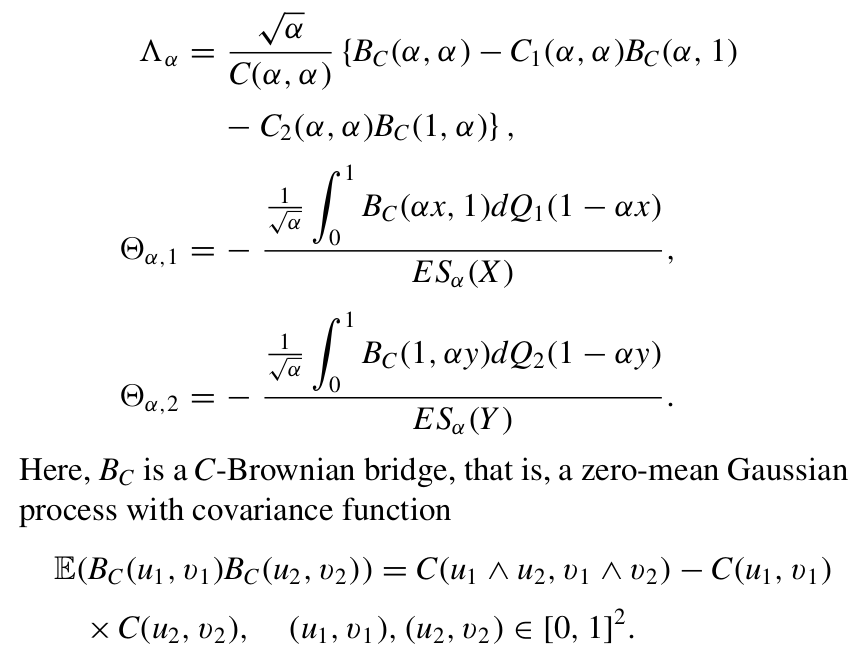
\includegraphics[width=0.5\textwidth]{ps1.png}
\end{figure}

\end{frame}



\begin{frame}
    \frametitle{fixed level}
Furthermore, if $k$ is a symmetric density with support $[-1,1]$ and bounded first derivative and the bandwidth $h=h(n)>0$ satisfies
$$
nh^2\to \infty \quad \text{and} \quad nh^4\to 0,
$$
then we have that, as $n \to \infty$,
$$
\sqrt{n\alpha}\suit{\frac{\hat{\rho}_{\alpha}-\tilde{\rho}_{\alpha}}{\rho_{\alpha}}}\stackrel{P}{\to} 0.
$$

\end{frame}


\begin{frame}
    \frametitle{Intermediate level}
When $\alpha$ is close to zero (but not extremely), it is often useful to model $\alpha$ as an intermediate sequence of $n$ in such a way that as $\alpha=\alpha_n\to 0$ and $n\alpha_n \to \infty$. 

For the study of an intermediate level $\alpha$, we need to control the tail behaviour of the distribution.
\end{frame}


\begin{frame}
    \frametitle{Assumption 2(intermediate level)}
\begin{itemize}
    \item For some $\gamma_j \in (0,1/2), \beta_j \le 0$ and function $A_j$ with a constant sign near infinity,
        $$
            \lim_{t\to \infty} \frac{1}{A_j(1/\bar{F}_j(t))}\suit{\frac{\bar{F}_j(tx)}{\bar{F}_j(t)}-x^{-1/\gamma_j}} = x^{-1/\gamma_j}\frac{x^{\beta_j/\gamma_j}-1}{\gamma_j \beta_j}.
        $$
    \item There exists a function $R:(0,\infty)^2\to [0,\infty]$ such that
            $$
                \lim_{t\to \infty} C(t^{-1}x,t^{-1}y)=R(x,y)
            $$
            and it has continuous first-order derivatives on a neighborhood of $(1,1)$.
    \item  The function $C$ has first-order derivatives on $(0,\delta)^2$ for some $\delta>0$ and as $t\to \infty$,
    $$
    \sup_{x,y \in (1-\delta,1+\delta)}\abs{C_i(t^{-1}x,t^{-1}y)-R_i(x,y)}\to 0.
    $$
\end{itemize}
    

\end{frame}
\end{document}